\documentclass{article}
\usepackage[utf8]{inputenc}
\usepackage{commath}
\usepackage{amsmath}
\usepackage{amssymb}
\usepackage{hyperref}
\usepackage{pgfplots}
\usepackage{physics}
\usepackage{ amssymb }
\usepackage[top=2.5cm, left=3cm, right=3cm, bottom=4.0cm]{geometry}
\usepackage{enumitem}
\pgfplotsset{width=10cm,compat=1.9}
\usepgfplotslibrary{external}
\tikzexternalize
\hypersetup{
    colorlinks=true,
    linkcolor=blue,
    filecolor=magenta,      
    urlcolor=cyan,
}

\usepackage{graphicx}
\urlstyle{same}

% make new command : single variable derivatives (i.e. non-partial)

\newcommand{\svd}[2]{\frac{\mathrm{d}#1}{\mathrm{d}#2} }
\newcommand{\svdi}[2]{\mathrm{d}#1/\mathrm{d}#2}
\newcommand{\svddi}[2]{\mathrm{d}^2#1/\mathrm{d}#2^2}
\newcommand{\svdd}[2]{\frac{\mathrm{d}^{2}{#1}}{\mathrm{d}{#2}^{2}} }

\newcommand{\pad}[2]{\frac{\partial#1}{\partial#2} }
\newcommand{\iig}[2]{\int #1 \mathrm{d}#2}
\newcommand{\vc}[1]{\mathbf{#1}}

\newcommand{\mybinom}[2]{\begin{bmatrix}#1 \\ #2 \end{bmatrix}}

\title{Python Battleships Review
}
\author{Chami Lamelas}
\date{August, 2021}

\begin{document}

\maketitle
\noindent In this document, I will review the Python syntax you will need to complete the battleships assignment. 

\section{Variables and Primitive Data Types}
In this section, I will talk about primitive data types, viewing data types in Python, and casting.

\subsection{Declaring Variables}
You can name a variable anything other than a Python reserved word. For example, this code creates an integer variable \texttt{int\_var} with value 5, a floating point variable \texttt{float\_var} with value 3.14, a string variable with value ``abc'', and a boolean variable with value \texttt{True}.
\begin{verbatim}
int_var = 5
float_var = 3.14
string_var = "abc"
bool_var = True
\end{verbatim}
Boolean variables can take on two values \texttt{True} or \texttt{\texttt{False}}.

\subsection{Viewing Data Types}
If you ever want to see the type of a variable, use the function ``type()'' which will return the type of the variable as a string. For example, we can print the types of the variables defined above. The \texttt{print} function will be discussed in more detail later.
\begin{verbatim}
print(type(int_var))
print(type(float_var))
print(type(string_var))
print(type(bool_var))
\end{verbatim}
This outputs
\begin{verbatim}
<class 'int'>
<class 'float'>
<class 'str'>
<class 'bool'>
\end{verbatim}

\subsection{Casting}
Strings are enclosed in quotation marks but can themselves contain numbers. To convert a string containing a number to a number, you need to cast it. In the code below, we have a string variable \texttt{str10} which holds the string ``10''. We then cast it to an integer to get the resulting integer variable \texttt{int10}.
\begin{verbatim}
str10 = "10"
int10 = int(str10)
\end{verbatim}
We can confirm that they indeed have different types by printing their types.
\begin{verbatim}
print(type(str10))
print(type(int10))
\end{verbatim}
This outputs
\begin{verbatim}
<class 'str'>
<class 'int'>
\end{verbatim}
For now, the \texttt{int()} function may seem useless, but all user input in Python is read as strings. Therefore, if you ever want to use user input as integers, you will have to cast them.\\\\
You can also cast from integers back to strings using the \texttt{str()} function. This code casts the integer variable \texttt{int20} to string variable \texttt{str20}. 
\begin{verbatim}
int20 = 20
str20 = str(int20)
\end{verbatim}
We can again print their types
\begin{verbatim}
print(type(int20))
print(type(str20))
\end{verbatim}
This outputs
\begin{verbatim}
<class 'int'>
<class 'str'>
\end{verbatim}
\texttt{str()} will be useful when we want to make integers as part of strings. This will be discussed in more detail in the string concatenation and printing sections below.

\subsection{Constants}
In other languages like Java and C, you can specify that some variables are constant and will never be changed after they are initialized. Python does not provide this capability, but you can signify variables as constants by making them entirely uppercase.
\begin{verbatim}
INCHES_IN_FOOT = 12
PI_APPROX = 3.14
\end{verbatim}
You are still able to change these variables later on, but uppercase is meant to signify to yourself or other programmers, that they should not be changed. Non-constant variables should be lowercase.

\newpage

\section{Integer and String Operations}
In this section, I will discuss some simple operations that can be performed on integers and strings.

\subsection{Integer Addition and Subtraction}
You can add two integers using (+) and subtract them using (-). In this code, we store the result of adding 10 and 5 in variable \texttt{a} and then print the result.
\begin{verbatim}
a = 10 + 5
print(a)
\end{verbatim}
This outputs
\begin{verbatim}
15
\end{verbatim}
We can also add two integer variables. This code creates two integer variables \texttt{b} and \texttt{c}, adds them together into variable \texttt{d}, then prints the result.
\begin{verbatim}
b = 6
c = -1
d = b + c
print(d)
\end{verbatim}
This outputs
\begin{verbatim}
5
\end{verbatim}
You can subtract integers in the same way, as in the following code.
\begin{verbatim}
f = 3 - 9
print(f)

g = 4
h = 2
i = g - h
print(i)
\end{verbatim}
This outputs
\begin{verbatim}
-6
2
\end{verbatim}
We can multiply integers in the same manner. However, division works slightly differently. Consider the following code
\begin{verbatim}
j = 6
k = 3
l = j/k
print(l)
\end{verbatim}
This outputs
\begin{verbatim}
2.0
\end{verbatim}
That is, \texttt{l} is a floating point variable. Similarly, if we perform the division
\begin{verbatim}
m = 2
n = 3
p = m/n
print(p)
\end{verbatim}
\texttt{p} is $0.\overline{6}$.

\subsection{Updating Shortcut}
It is very common that you will be updating a variable to be $n$ more or $n$ less than its current value. For example, suppose you have a variable \texttt{x} that is 10. Later on, suppose you want to update the variable \texttt{x} to be 5 more than it's current value. You can write
\begin{verbatim}
x = x + 5
\end{verbatim}
which properly updates \texttt{x} to be 15. However, Python provides a shortcut
\begin{verbatim}
x += 5
\end{verbatim}
Python provides similar shortcuts for subtraction, multiplication, and division. Instead of writing
\begin{verbatim}
y = y - 5
y = y * 5
y = y / 5
\end{verbatim}
we can write
\begin{verbatim}
y -= 5
y *= 5
y /= 5
\end{verbatim}

\subsection{String Concatenation}
If you want to combine strings one after another, you can concatenate them using the + operator. Suppose we have the following string variables
\begin{verbatim}
first_name = "John"
last_name = "Smith"
\end{verbatim}
Now, we want to combine them into a new string variable \texttt{full\_name} that will be made up of the first name followed by the last name separated by a space. We can create this variable as follows
\begin{verbatim}
full_name = first_name + " " + last_name
\end{verbatim}
If we print this, it will display
\begin{verbatim}
John Smith
\end{verbatim}
It is important to note that we do not have to declare a space `` '' as a variable. Whenever a string appears in code surrounded by quotation marks, it is called a string literal. We can concatenate string variables and literals in any order.\\\\
We cannot concatenate a string with an integer. For example, suppose we again had the string variables
\begin{verbatim}
first_name = "John"
last_name = "Smith"
\end{verbatim}
But we also had John Smith's age
\begin{verbatim}
age = 45
\end{verbatim}
Now, suppose we want to create a string variable that has the first name followed by the last name, followed by the age, each separated by a space. First, try concatenating them as is with +:
\begin{verbatim}
full_name_and_age = first_name + " " + last_name + " " + age
\end{verbatim}
This will generate an error
\begin{verbatim}
TypeError: can only concatenate str (not "int") to str
\end{verbatim}
\texttt{str} is the Python string data type and \texttt{int} is the integer data type. This error is telling us that we have a variable with the wrong type in the concatenation. To fix this issue, we need to cast age to a string before concatenating it. 
\begin{verbatim}
full_name_and_age = first_name + " " + last_name + " " + str(age)
\end{verbatim}
This code will put the first name, followed by a space, then the last name, then another space, then the string representation of the age into \texttt{full\_name\_and\_age}. Note that we do not need to store \texttt{str(age)} in a variable, we can do it in the declaration of \texttt{full\_name\_and\_age}.\\\\
For another example, suppose we have three integers storing the year, month, and date of someone's birthday.
\begin{verbatim}
bday_year = 2020
bday_month = 12
bday_day = 11
\end{verbatim}
Suppose we want to turn them into a MM/dd/yyyy string. That is, the month followed by a /, then the day, another /, and then the year (with no spaces!). We can do this with the following code
\begin{verbatim}
bday_str1 = str(bday_month) + "/" + str(bday_day) + "/" + str(bday_year)
\end{verbatim}
Note that we have to cast each of the integer variables to strings before putting slashes between them.\\\\
We could also easily create a yyyy-MM-dd date string from these same three variables
\begin{verbatim}
bday_str2 = str(bday_year) + "-" + str(bday_month) + "-" + str(bday_day)
\end{verbatim}

\section{Control Flow I: Conditional Statements}
In thie section, I will discuss boolean conditions and how they are used to build if-elif-else statements.

\subsection{Comparison Operators}
Integers can be compared using a set of operators
\begin{itemize}
    \item \texttt{<} : less than
    \item \texttt{>} : greater than
    \item \texttt{<=} : less than or equal to
    \item \texttt{>=} : greater than or equal to
    \item \texttt{==} : equal to (this applies to both strings and integers)
    \item \texttt{!=} : not equal to
\end{itemize}
Note the difference between the equality operator \text{==} and the assignment operator \text{=}.

\subsection{Primitive Boolean Conditions}
A boolean expression is any expression that evaluates to \texttt{True} or \texttt{\texttt{False}}. We can use comparison operators to build boolean expressions. For example, 
\begin{verbatim}
b1 = 2 < 5
b2 = 2 > 5
b3 = 3 >= 1
b4 = 3 <= 1
b5 = 2 == 1
b6 = 2 != 1
\end{verbatim}
\texttt{b1} to \texttt{b6} are all boolean variables. Printing them outputs
\begin{verbatim}
True
False
True
False
False
True
\end{verbatim}

\subsection{Building Compound Boolean Conditions}
You can build more complex boolean conditions using \texttt{and} and \texttt{or}. Suppose that \texttt{b1} and \texttt{b2} are boolean expressions.\\\\
The compound expression \texttt{b1 and b2} is evaluated in this manner
\begin{enumerate}
    \item Check if \texttt{b1} is \texttt{True}. If so, go to step 2. Otherwise, \texttt{b1 and b2} is \texttt{False}.
    \item Check if \texttt{b2} is \texttt{True}. If so, \texttt{b1 and b2} is \texttt{True}. Otherwise, \texttt{b1 and b2} is \texttt{False}.
\end{enumerate}
The compound expression \texttt{b1 or b2} is evaluated in this manner
\begin{enumerate}
    \item Check if \texttt{b1} is \texttt{True}. If so, \texttt{b1 and b2} is \texttt{True}. Otherwise, go to step 2.
    \item Check if \texttt{b2} is \texttt{True}. If so, \texttt{b1 and b2} is \texttt{True}. Otherwise, \texttt{b1 and b2} is \texttt{\texttt{False}}.
\end{enumerate}
When building more complex compound expressions with nested \texttt{and}s and \texttt{or}s, make sure to enclose expressions in parenthesis to ensure expressions are evaluated in the way you want.\\\\
For example, suppose someone is allowed to attend an event if they are at least 18 or if they are at least 16 with an adult. For simplicity, suppose we have already determined the age and companion in an integer variable \texttt{age} and boolean variable \texttt{with\_adult} respectively. We can construct a boolean variable \texttt{allowed} that stores whether the person is allowed into the event
\begin{verbatim}
allowed = (age >= 18) or (age >= 16 and with_adult)
\end{verbatim}
Note here that we collect the two separate ``allowed'' conditions in parenthesis. \texttt{(age >= 18)} means the person is an adult and \texttt{(age >= 16 and with\_adult)} means the person is at least 16 and accompanied by an adult. One could ask, why don't we need to write
\begin{verbatim}
allowed = (age >= 18) or (age < 18 and age >= 16 and with_adult)
\end{verbatim}
However, as noted in the evaluation order for \texttt{or} listed above, the second expression will only be evaluated if the first expression is false. In this case, if we get to evaluating \texttt{age < 18 and age >= 16 and with\_adult}, that means \texttt{(age >= 18)} evaluated to \texttt{False} already. Therefore, \texttt{(age < 18)} is redundant and the second expression can be simplified to \texttt{(age >= 16 and with\_adult)}.

\subsection{Negating Boolean Conditions}
In the section on comparison operators, we introduced the not equals operator \texttt{!=}. However, we can also negate any boolean expression (or variable) with the keyword \texttt{not}. For example, we can create the boolean variable \texttt{rejected} as the opposite of \texttt{allowed}.
\begin{verbatim}
rejected = not allowed
\end{verbatim}
Or, we can write it as the negation of the boolean expression used to define \texttt{allowed}
\begin{verbatim}
rejected = not ((age >= 18) or (age >= 16 and with_adult))
\end{verbatim}
It is important to note here that we want to negate the entire boolean expression \texttt{(age >= 18) or (age >= 16 and with\_adult)} so we enclose it in parenthesis before applying \texttt{not} to it.

\subsection{if-elif-else Statements}
We can use boolean expressions to build \texttt{if-elif-else} statements. A simple \texttt{if} statement can be constructed
\begin{verbatim}
if allowed:
    print("Welcome to the event!")
\end{verbatim}
This code will print ``Welcome to the event!'' whenever the boolean variable \texttt{allowed} is \texttt{True}. We do not need to write \texttt{allowed == True} because \texttt{allowed} on its own evaluates to a boolean value and can be verified by an \texttt{if} statement. This is known as \textit{boolean zen}.\\\\
The print statement is known as the body of the if statement. All of the lines in the body of the if statement must be indented by 1 from the if statement. The body of the if statement is executed when the boolean condition is \texttt{True}.\\\\
The boolean condition check by the if statement does not need to be stored in a variable. For example, the above if statement is identical to
\begin{verbatim}
if (age >= 18) or (age >= 16 and with_adult):
    print("Welcome to the event!")
\end{verbatim}
Now, suppose that we want to print ``Sorry, you cannot enter!'' in the event if someone does not match the criteria to enter. We can implement this with an \texttt{else} statement.
\begin{verbatim}
if (age >= 18) or (age >= 16 and with_adult):
    print("Welcome to the event!")
else:
    print("Sorry, you cannot enter!")
\end{verbatim}
Like with an if statement, the body of the else statement must be indented by 1 tab from the else.\\\\
Now, suppose that we want to print ``Welcome to the event!'' if someone is an adult, ``Welcome to the event, stay with your adult!'', if someone is at least 16 with an adult, and ``Sorry, you cannot enter!'' otherwise. We can implement this with an \texttt{if-elif-else} statement.
\begin{verbatim}
if age >= 18:
    print("Welcome to the event!")
elif age >= 16 and with_adult:
    print("Welcome to the event, stay with your adult!")
else:
    print("Sorry, you cannot enter!")
\end{verbatim}
Note that we have broken up the compound boolean condition used to define \texttt{allowed} because we require two different print statements. An \texttt{elif} statement is only checked if all preceding \texttt{if} and \texttt{elif} statements have evaluated to \texttt{\texttt{False}}. The body of the \texttt{elif} statement, like \texttt{if} and \texttt{else} statements must be indented by 1 tab. The body will only be run if the \texttt{elif} condition is \texttt{True}. The \texttt{else} body is executed if all preceding \texttt{if} and \texttt{elif} statements were checked and evaluated to \texttt{\texttt{False}}.\\\\
Here, a more complicated \texttt{if-elif-else} statement is used to print the appropriate education based on age.
\begin{verbatim}
if age < 5:
    print("Pre-school")
elif age < 13:
    print("Middle school")
elif age < 18:
    print("High school")
elif age <= 22:
    print("College")
else:
    print("Post-college")
\end{verbatim}
Suppose we had instead implemented this with
\begin{verbatim}
if age < 5:
    print("Pre-school")
elif age >= 5 and age < 13:
    print("Middle school")
elif age >= 13 and age < 18:
    print("High school")
elif age >= 18 and age <= 22:
    print("College")
else:
    print("Post-college")
\end{verbatim}
This is equivalent, but redundant. In order to reach \texttt{age >= 5 and age < 13}, \texttt{age < 5} needed to have evaluated to \texttt{\texttt{False}}. Or in other words, \texttt{age >= 5} would always evaluate to \texttt{True} if \texttt{age < 5} was passed. The conditions \texttt{age >= 13} and \texttt{age >= 18} appear in the third and fourth \texttt{elif} statements are redundant for the same reason.\\\\
Now, suppose we had implemented this with 
\begin{verbatim}
if age < 5:
    print("Pre-school")
if age < 13:
    print("Middle school")
if age < 18:
    print("High school")
if age <= 22:
    print("College")
else:
    print("Post-college")
\end{verbatim}
Consider the case where \texttt{age = 12}. This would print
\begin{verbatim}
Middle school
High school
College
\end{verbatim}
This is because a list of \texttt{if} statements do not work the same as a list of \texttt{elif} statements. Each \texttt{if} statement will be checked regardless of whether \texttt{if} statements are evaluated to \texttt{True}. In the case where \texttt{age = 12}, \texttt{age < 13}, \texttt{age < 18}, and \texttt{age <= 22} all evaluate to \texttt{True}. Hence, the three corresponding education levels are printed.

\subsection{Ternary Operator (if-else shortcut)}
It is quite common that we have a variable \texttt{x} and want to set it to one value if a condition holds and another otherwise. Suppose for instance, we want \texttt{age\_group} to be ``adult'' if another variable \texttt{age} is at least 18 and ``child'' otherwise. As of now, we would write this code.
\begin{verbatim}
age_group = ""
if age >= 18:
    age_group = "adult"
else:
    age_group = "child"
\end{verbatim}
Since this is so common, Python has provided a shortcut.
\begin{verbatim}
age_group = "adult" if age >= 18 else "child"
\end{verbatim}
This code will set \texttt{age\_group} to ``adult'' if \texttt{age >= 18} and to ``child'' otherwise (as desired). This is quite useful because it allows us to omit the initialization step of setting \texttt{age\_group = ""} and reduces our code to one line. In general a ternary operator has the form
\begin{verbatim}
(true result) if (condition to check) else (false result)
\end{verbatim}
Note that there are no colons involved in a ternary operator as with regular \texttt{if} and \texttt{else} statements.

\section{Control Flow II: Loops}
In this section, I will discuss the second primary component of controlling the flow of programs: loops. 

\subsection{While Loops}
A while loop can be used to run a body of code while a condition is true. For example, suppose we are given a number $n = 2^k$ and we want to calculate $k$. We can use a while loop to do this with the following code assuming we have defined some variable \texttt{n}.
\begin{verbatim}
k = 0
while n > 1:
    k += 1
    n /= 2
\end{verbatim}
In this loop, the code
\begin{verbatim}
k += 1
n /= 2
\end{verbatim}
will be executed while \texttt{n > 1}. Once \texttt{n <= 1}, then the code following the loop will be executed. It is important to note that we must declare \texttt{k=0} outside of the loop as it is updated at each loop iteration until we reach \texttt{n=1}.\\\\
For another example, suppose we want to compute $a^b$. We can do this with the following code
\begin{verbatim}
result = a
i = 1
while i < b:
    result *= a
    i += 1
\end{verbatim}
In this loop, the code
\begin{verbatim}
result *= a
i += 1
\end{verbatim}
will be executed while \texttt{i < b}. In the previous code, \texttt{n} serves as the iterating variable. We reduce \texttt{n} by 2 until it is 1 and count the number of divisions that were required in \texttt{k}. In this code, the iterating variable is \texttt{i}. We multiply \texttt{result} by \texttt{a} until \texttt{i} has reached \texttt{b}. Again, it is important to note that since they are used inside the \texttt{while} loop, \texttt{result} and \texttt{i} are declared outside the loop.

\subsection{For Loops}
It is very common that we loop from $a$ to $b$ one number at a time. This gave rise to the \texttt{for} loop. The \texttt{for} loop can be used to provide an alternate implementation for computing $a^b$.
\begin{verbatim}
result = a
for i in range(1,b):
    result *= a
\end{verbatim}
\texttt{range(m,n)} yields a sequence of integers $m,m+1,\dots,n-1$. The statement \texttt{for i in range(1,b)} will then iterate over each \texttt{i} in the sequence \texttt{1,2,...,b-1}.\\\\
It is even more common for you to iterate on a range \texttt{0,1,...,n-1}. This can be done with the statement \texttt{for i in range(n)}. For example, we can sum the elements from 1 to \texttt{n} with the following code.
\begin{verbatim}
sum = 0
for i in range(n):
    sum += i + 1
\end{verbatim}
Due to the \texttt{for} loop, \texttt{while} loops are generally reserved for checking more complex boolean conditions. For example, it is commonly used for waiting for valid user input. 

\subsection{Nested Loops}
You can also nest loops within each other as a loop can be thought of as any other code to be executed in the body of another loop. For instance, suppose we want to print a 12 times table. That is, we want to print $1*1$, $1*2$, up to $1*12$ and similar for 2 through 12. This can be done with the following code
\begin{verbatim}
for i in range(1,13):
    for j in range(1,13):
        print(i*j)
\end{verbatim}
This will print
\begin{verbatim}
1
2
...
12
2
4
...
24
3
6
...
36
...
12
24
...
144
\end{verbatim}
It is important to note here that since the iterating variable \texttt{i} is used by the outer loop, we need a new iterating variable in the inner loop \texttt{j}. For each iterating \texttt{i} of the outer loop, we run the inner loop from \texttt{j=1} to \texttt{j=12}. In the innermost loop, we print \texttt{i*j}. At first \texttt{i=1,j=1} then \texttt{i=1,j=2} until \texttt{i=1,j=13} and the inner loop ends. Then, we move to the second iteration of the outer loop where we start at \texttt{i=2,j=1}, continue to \texttt{i=2,j=13} and repeat the process until \texttt{i=13} and the outer loop is over.

\section{Printing}
In this section, I will discuss the \texttt{print} function in more detail.

\subsection{Printing Multiple Data Types}
Until now, we have been printing different data types by just passing them into \texttt{print}. For example, in this code we print an integer value, a floating point value, a boolean value, and a string value.
\begin{verbatim}
print(1)
print(2.3)
print(True)
print("hi")
\end{verbatim}
Suppose we have the following variables
\begin{verbatim}
first_name = "John"
last_name = "Smith"
age = 13
\end{verbatim}
and we want to print ``John Smith is 13 years old!'' using the variables above. We can do this by building a string to be printed
\begin{verbatim}
pstr = first_name + " " + last_name + " is " + str(age) + " years old!"
\end{verbatim}
And then print it to see the desired result
\begin{verbatim}
print(pstr)
\end{verbatim}
However, we do not need to build the result of the string concatenation into a string before printing it. We can just perform the concatenation when calling print:
\begin{verbatim}
print(first_name + " " + last_name + " is " + str(age) + " years old!")
\end{verbatim}

\subsection{The Newline Character (\textbackslash n)}
The character \textbackslash n is a special string character that can be used to separate a string onto multiple lines. For example, suppose we want a string formatted onto two lines that would look like this
\begin{verbatim}
Hello
World!
\end{verbatim}
This string would be stored in a variable like this
\begin{verbatim}
hw = "Hello\nWorld!"
\end{verbatim}
If we then printed \texttt{hw}, we would see ``Hello'' and ``World!'' on separate lines as above.

\subsection{Printing on the Same Line}
Note that if we write
\begin{verbatim}
print(1)
print(2.3)
print(True)
print("hi")
\end{verbatim}
That this outputs
\begin{verbatim}
1
2.3
True
hi
\end{verbatim}
Or in other words, each print statement places its input on a newline. Suppose we wanted to place 1 and 2.3 on the same line. To do so, when we print 1, we will need to specify that we don't want the next print to be placed on a new line. This is done by using the \texttt{end} parameter in \texttt{print()}.
\begin{verbatim}
print(1, end="")
print(2.3)
\end{verbatim}
The output of this code is
\begin{verbatim}
12.3
\end{verbatim}
The parameter \texttt{end} specifies what should be printed at the end of the current line after the input you passed in. By default, when you call \texttt{print}, \texttt{end} can be thought of as already being set to \texttt{\textbackslash n}. By specifying \texttt{end} as the empty string \texttt{""}, then nothing is printed after 1 which means that the subsequent call \texttt{print(2.3)} will place 2.3 directly after 1. Alternatively, suppose we want to print 1 followed by a space, then 2.3. We can do this with the following code
\begin{verbatim}
print(1, end=" ")
print(2.3)
\end{verbatim}

\newpage

\section{Lists}
In this section, I will be discussing the list data structure and some of the operations one can perform on it.

\subsection{Creating Lists}
One can create an empty list \texttt{ls} in two ways
\begin{verbatim}
ls = list()
\end{verbatim}
or
\begin{verbatim}
ls = []
\end{verbatim}
You can also create a list with some elements already in it. For instance, suppose you want to create a list with elements 1, 2, and 3 in that order. We can do this with the following code
\begin{verbatim}
ls = [1, 2, 3]
\end{verbatim}
Now, suppose you want to create a list with 10 zeros. Python provides a shortcut to do this using the multiplication operator
\begin{verbatim}
ls = [0]*10
\end{verbatim}
This is equivalent to writing out
\begin{verbatim}
ls = [0, 0, 0, 0, 0, 0, 0, 0, 0, 0]
\end{verbatim}

\subsection{Indexing a List}
Python lists are indexed from 0 to 1 less than the length of the list. The length of a list \texttt{ls} can be found using the \texttt{len} function. For instance, this code will print 3.
\begin{verbatim}
ls = [1, 2, 3]
print(len(ls))
\end{verbatim}
You can index elements of a list using the \texttt{[ ]} operator following the list name. For example \texttt{ls[0]} is 1, \texttt{ls[1]} is 2, and \texttt{ls[2]} is 3. You are able to pass in any value between 0 and \texttt{len(ls)-1} into \texttt{[ ]}.\\\\
You can use \texttt{[ ]} to change the element at an index in the list. For example, suppose we want to change
\begin{verbatim}
ls = [1, 2, 3]
\end{verbatim}
to
\begin{verbatim}
ls = [1, 5, 3]
\end{verbatim}
without creating an entirely new list. We can do this with the following code
\begin{verbatim}
ls[1] = 5
\end{verbatim}
We can think of \texttt{ls[i]} as a new variable essentially. The following example will illustrate this. Suppose that we have a list \texttt{ls} and we want to negate all of the elements in the list. This can be done using the loop
\begin{verbatim}
for i in range(len(ls)):
    ls[i] *= -1
\end{verbatim}
Python provides support for printing a list, so you can call \texttt{print(ls)} to see the desired result.
\begin{verbatim}
[-1, -2, -3]
\end{verbatim}

\subsection{Adding to a List}
You can add new elements to the end of a list using the \texttt{append()} function on a list. For example, if I have the list
\begin{verbatim}
ls = [1, 2, 3]
\end{verbatim}
I can add 4 to the end of it by calling
\begin{verbatim}
ls.append(4)
\end{verbatim}

\subsection{Two-dimensional Lists}
Python, by default, does not have a separate data structure for two dimensional lists (or matrices). We can represent two dimensional lists as a list of lists. Each list can be thought of as a row of a two dimensional list. Suppose I want to represent the 3x3 identity matrix
\begin{verbatim}
1 0 0
0 1 0
0 0 1
\end{verbatim}
This can be done with the following code
\begin{verbatim}
identity = [[1, 0, 0],[0, 1, 0],[0, 0, 1]]
\end{verbatim}
Each of the elements of \texttt{identity} is itself a list, as we can see here
\begin{verbatim}
print(type(identity[0]))
print(type(identity[1]))
print(type(identity[2]))
\end{verbatim}
This outputs
\begin{verbatim}
<class 'list'>
<class 'list'>
<class 'list'>
\end{verbatim}
You are allowed to space out the rows of \texttt{identity} so it looks more like a matrix
\begin{verbatim}
identity = [
    [1, 0, 0],
    [0, 1, 0],
    [0, 0, 1]
]    
\end{verbatim}
Since we know that a two dimensional list is really a list of lists, we will need to index into two different lists to see a particular element. For example, suppose you want to retrieve the upper left element of the identity matrix. We know that this is in the first column of the first row. We can use this logic to identify the two list indexes we have to make. First, we want to get the first row in \texttt{identity}. This can be retrieved with \texttt{identity[0]}. Now, we want to get the first column in this row. This can be retrieved by getting the first element of \texttt{identity[0]} with \texttt{identity[0][0]}. Printing \texttt{identity[0][0]} displays 1 as expected.\\\\
In general, \texttt{identity[i][j]} produces the element that is stored in the $j$th column of the $i$th row. Applying the logic from above, we first get the $i$th row with \texttt{identity[i]} and then get the $j$th element of it with \texttt{identity[i][j]}. Note that the number of rows in a two dimensional list is \texttt{len(identity)-1}. It is also important to note that when we think of matrices, we assume that each row has the same number of columns. Since a Python two dimensional list is really a list of lists, each of those lists could have different lengths. Therefore, the number of elements (or columns) of $i$th row is \texttt{len(identity[i])}. Therefore, the above indexing only applies for $i=0,1,\dots,$\texttt{len(identity)-1} and $j=0,1,\dots,$\texttt{len(identity[i])-1}.\\\\
If we print a two dimensional list, the output will not look like a matrix. For instance, \texttt{print(identity)} will yield
\begin{verbatim}
[[1, 0, 0], [0, 1, 0], [0, 0, 1]]
\end{verbatim}
However, we can use a combination of nested loops and \texttt{print()} with different \texttt{end} values to print a matrix that looks like
\begin{verbatim}
1 0 0
0 1 0
0 0 1
\end{verbatim}
We need nested loops because we will have an outer loop that iterates over each row and then an inner loop that iterates over each column. We want to print each element in a row on the same line, but keep rows separated.
\begin{verbatim}
for i in range(3):
    for j in range(3):
        print(identity[i][j],end=" ")
    print("")
\end{verbatim}
The outer loop iterates over each row \texttt{i}. The inner loop iterates over each column \texttt{j} in row \texttt{i}. Within the inner loop, we end each print with \texttt{" "} as opposed to printing onto a newline. After we print a row, \texttt{print("")} will print a newline and nothing else. That way, future prints in the following row will be on a newline. It is important to note that this technically prints a space at the end of each row even though it isn't apparent in the output.

\subsection{The \texttt{range()} Function (What does \texttt{for in} really mean?)}
Recall our syntax for writing a \texttt{for} loop in Python: 

\begin{verbatim}
for i in range(start,stop):
    ...
\end{verbatim}
\texttt{range()} is actually a function that produces a list-like sequence of numbers depending on the supplied parameters. The parameters of \texttt{range()} are:

\begin{itemize}
    \item \texttt{start} : the start of the sequence of numbers that \texttt{range()} produces. If this is not provided, it is set to 0.
    \item \texttt{stop} : the number that is the last number in the sequence that \texttt{range()} produces plus \texttt{step}. That is, it is not included in the produced sequence.
    \item \texttt{step} : the number that determines the step between the elements of the sequence that \texttt{range()} produces. If this is not provided, it is set to 1. 
\end{itemize}
Here are three examples that demonstrate the three common ways this function is used:
\begin{itemize}
    \item \texttt{range(5)} : this produces the sequence $0,1,2,3,4$. If only one parameter is provided to \texttt{range()}, it is interpreted as the \texttt{stop} parameter. \texttt{start} is 0 and \texttt{step} is 1. Note \texttt{stop = 5} is not included in the sequence.
    
    \item \texttt{range(1,4)} : this produces the sequence $1,2,3$. Here the \texttt{start} and \texttt{stop} parameters are provided, and \texttt{step} is 1. Again, \texttt{stop = 4} is not included in the sequence.
    
    \item \texttt{range(5,-1,-1)} : this produces the sequence $5,4,3,2,1,0$. Here all three parameters are provided. We specify that we want to decrease by having \texttt{stop < start} and a \texttt{step} of -1. We can see that this is indeed the step of the sequence above. Again, \texttt{stop = -1} is not included in the sequence.
\end{itemize}
It turns out that \texttt{for e in s} just iterates over the elements \texttt{e} of a sequence \texttt{s}. We can see that this is indeed true in the case of \texttt{range()} based on the above discussion. In fact, we can use it to just iterate over the elements of a list without explicitly indexing the list. That is, we can now write a \texttt{for} loop that mimics ``for each element in list l'' as opposed to ``for each index in list l''. For example, suppose we want to write a function that sums the elements of a list \texttt{l}. We would originally write this as:
\begin{verbatim}
def sum_list_original(l):
    s = 0
    for i in range(len(l)):
        s += l[i]
    return s
\end{verbatim}
Now that we know \texttt{for e in s} iterates over the elements \texttt{e} of a sequence \texttt{s}, we can use this to define a newer version of this function:
\begin{verbatim}
def sum_list_new(l):
    s = 0
    for e in l:
        s += e
    return s
\end{verbatim}
Now, it is important to note that you cannot replace every loop that goes over a list using indices with one that goes over the elements. To sum all of the elements of a list, the indices are not needed. However, suppose we wanted to write a function to see if two lists \texttt{l1,l2} of equal length are equal. We still need to compare the elements at each index of the two lists as follows:
\begin{verbatim}
def list_equals(l1,l2):
    for i in range(len(l1)):
        if l1[i] != l2[i]:
            return False
    return True
\end{verbatim}


\section{Mutability}
List variables have different properties than variables of primitive types such as integers, booleans, strings, and floating point numbers. 

\subsection{Idea of a Pointer}
In memory, a list variable can be thought of as a pointer to an array of adjacent cells. For example, suppose we create a list
\begin{verbatim}
ls = [1, 2, 3, 4, 5]
\end{verbatim}
The variable \texttt{ls}'s memory representation looks something like Figure 1.

\newpage

\begin{figure}[hbt]
    \centering
    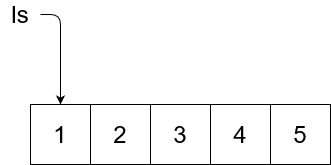
\includegraphics[width=0.3\textwidth]{pointer_diagram_1.png}
    \caption{Memory Diagram for \texttt{ls}}
    \label{fig:my_label}
\end{figure}
\noindent We can think of \texttt{ls} as more simply storing an address in memory where the actual data (1, 2, 3, 4, 5) is stored. The arrow in Figure 1 indicates that \texttt{[1, 2, 3, 4, 5]} is not directly associated with \texttt{ls} but it is stored at an index known by \texttt{ls}. An alternate diagram is shown in Figure 2.

\begin{figure}[hbt]
    \centering
    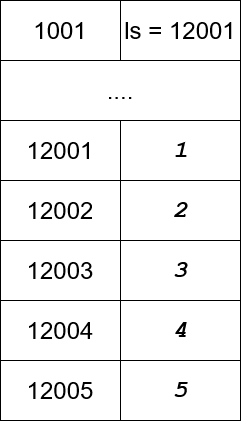
\includegraphics[width=0.2\textwidth]{pointer_diagram_2.png}
    \caption{Alternate Memory Diagram for \texttt{ls}}
    \label{fig:my_label}
\end{figure}
\noindent In this diagram, the variable \texttt{ls} is stored at some memory location labelled 1001. The value of \texttt{ls} is actually another memory address labelled 12001. 12001 through 12005 store the 5 elements in the list (these are italicized to convey that they are integer data not other memory locations). When we index \texttt{ls} with \texttt{ls[i]} Python will go to the location \texttt{ls} refers to (12001 in Figure 2) and then move over by \texttt{i}. For example, when Python executes \texttt{ls[2]}, it will go first to 12001, then move over by 2 to 12003. We can now read or update the data at the memory location 12003.\\\\
Therefore, we can see that we are changing the data that is in the list without pointing \texttt{ls} to some other memory location. \texttt{ls} remains at 12001 while we can change the data in locations 12001 to 12005.

\subsection{Tuple, the Immutable List}
Python provides an immutable collection known as a tuple. You cannot change the elements of a tuple, which makes it immutable. We can create a tuple using parenthesis as opposed to square brackets.
\begin{verbatim}
tup = (1,2,3,4,5)
\end{verbatim}
We can print its type which is
\begin{verbatim}
<class 'tuple'>
\end{verbatim}
We can access the elements of \texttt{tup} in the same way as with a list. For example, \texttt{print(tup[1])} prints 2. It is important to note that a single element tuple has special syntax:
\begin{verbatim}
stup = (1,)
\end{verbatim}
That is, you need to place a comma after the one and only element in the tuple. Tuples are generally used to collect grouped information that will not be changed. For instance, we can easily represent a $(x,y)$ point in $\mathbb{R}^2$ as a 2-element tuple. 

\subsection{Copying Lists and the Shallow Copy}
Now that we have introduced that a list is a mutable data structure, what happens when we execute the following code?
\begin{verbatim}
ls = [1,2,3,4,5]
ls2 = ls
\end{verbatim}
Recall Figure 2 on page 15. \texttt{ls} is really just a memory location 12001. Therefore, \texttt{ls2 = ls} simply copies the value of \texttt{ls} into \texttt{ls2}. Thus, \texttt{ls2} is also 12001. We can represent this in cells in Figure 3, assuming that \texttt{ls2} is stored in a memory cell labelled 1002.
\begin{figure}[hbt]
    \centering
    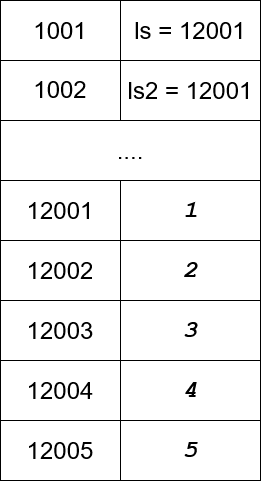
\includegraphics[width=0.2\textwidth]{pointer_diagram_3.png}
    \caption{Memory Diagram for \texttt{ls} and \texttt{ls2}}
    \label{fig:my_label}
\end{figure}\\
A graphical interpretation of this akin to Figure 1 can be found on the following page in Figure 4. Therefore, we can now see that \texttt{ls} and \texttt{ls2} point to the same chunk of data in memory. Thus, if we run \texttt{ls2[2] = 0} then the data at memory cell 12003 will now be 0. Therefore, when we run \texttt{ls[2]}, we will get 0. Updates to \texttt{ls2} will now affect the data pointed to by \texttt{ls} (as it is the \textit{same data}).

\begin{figure}[hbt]
    \centering
    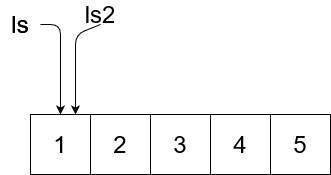
\includegraphics[width=0.35\textwidth]{pointer_diagram_4.png}
    \caption{Graphical Memory Diagram for \texttt{ls} and \texttt{ls2}}
    \label{fig:my_label}
\end{figure}
\noindent What we really want when we copy data is to have something that looks like Figure 5.

\newpage

\begin{figure}[hbt]
    \centering
    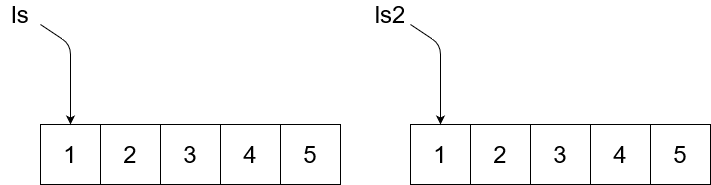
\includegraphics[width=0.7\textwidth]{pointer_diagram_5.png}
    \caption{A True Copy of \texttt{ls}}
    \label{fig:my_label}
\end{figure}

\noindent That is, we have \texttt{ls} and \texttt{ls2} both referring to lists with elements \texttt{[1,2,3,4,5]} stored separately. An example memory set up is given in Figure 6 which is akin to figures 2 and 3.\\\\
Now, suppose we execute the following code. What will it output?
\begin{verbatim}
ls2[2] = 0
print(ls[2])
\end{verbatim}
This will output 3. That is, the data pointed to by \texttt{ls} was not updated. Why is this? Remember, when we call \texttt{ls2[2] = 0}, Python will go to 22001 (see Figure 6), move down by 2 to 22003, and update the data at cell 22003 to 0. Then, when we run \texttt{print(ls[2])}, we go to 12001, move down by 2 to 12003 and print the data at cell 12003 which is 3. Note that the memory addresses of \texttt{ls} and \texttt{ls2} (12001 and 22001 respectively) were chosen for no particular reason. When we perform a copy akin to figure 4, we call this a \textit{shallow copy}. When we have two separate lists as in Figure 5, we call it a \textit{deep copy}. 
\begin{figure}[hbt]
    \centering
    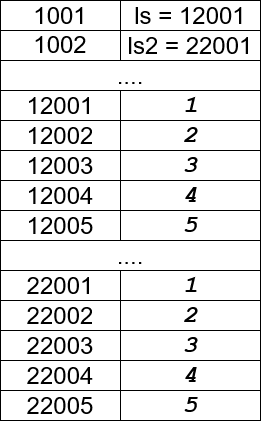
\includegraphics[width=0.3\textwidth]{pointer_diagram_6.png}
    \caption{A True Copy of \texttt{ls}}
    \label{fig:my_label}
\end{figure}\\

\newpage

\subsection{What about Primitives? Are they Mutable?}
Primitives are variables of primitive data types. That is, of types \texttt{bool}, \texttt{int}, or \texttt{float}. For example,
\begin{verbatim}
int_var = 5
float_var = 3.14
bool_var = True
\end{verbatim}
When we ask the program for \texttt{int\_var}, we just get back the integer stored at some memory location. In essence, it is not a pointer that points to some cell that can be edited. It is the same for \texttt{float} and \texttt{bool} type variables as well. Suppose we wrote the following code.
\begin{verbatim}
int_var = 5
int_var2 = int_var
\end{verbatim}
This will copy the contents of \texttt{int\_var} into \texttt{int\_var2}. That is, they will both be 5. The only way we can change \texttt{int\_var2} is to assign it to something else which will have no effect on \texttt{int\_var}.

\section{Functions}
In this section, I will cover the purpose and components of functions, different types of functions, and how they will be invoked (or called).

\subsection{Why do we need functions? (Introduction to Modularity)}
In math, a function takes an input from some domain and returns an output in some range. We can create the equivalent of various mathematical functions. For instance, we could create the equivalent of $y = f(x) = 3x + 5$.
\begin{verbatim}
def y(x):
    return 3*x + 5
\end{verbatim}
The Python keyword \texttt{def} creates a new function named \texttt{y} that takes a single input \texttt{x}. The Python keyword \texttt{return} causes the function to end and outputs the result of the expression that follows it (in this case the expression \texttt{3*x + 5} evaluated at whatever \texttt{x} is). We can retrieve \texttt{y} values that correspond to various \texttt{x} by invoking or calling \texttt{y(x)}. For instance, \texttt{print(y(3))} prints 14.\\\\
We can also create functions with multiple parameters. For instance, suppose we wanted to create the equivalent of the mathematical function $z = f(x,y) = 3x + 2y + 5$. This can be done with the following code.
\begin{verbatim}
def z(x,y):
    return 3*x + 2*y + 5
\end{verbatim}
This function has two parameters \texttt{x} and \texttt{y}. We can call it with 2 parameters and present the result. For instance, \texttt{print(z(3,7))} prints 28.\\\\
In programs, we can think of a function as any kind of action while variables correspond to quantities. This is because functions in programs do not have to take input and do not have to return output. Functions can edit our input or can display output to the user via the console or a graphical user interface.\\\\
We could technically implement our programs without any functions. However, by breaking up all the actions required to implement a larger program into functions, it will make our programs easier to read and debug. We can test functions separately and make sure they work before incorporating them together. This is known as \textit{unit testing}. By thinking of functions as the equivalent of actions, we can write the larger program assuming that the actions are already implemented. For instance, suppose we wanted to write a program that repeatedly prompts a user for information on a person (name, age, gender, etc.) and then adds that information to a database. We could come up with an algorithm in English that is something like
\begin{verbatim}
while (the user is not done)
    (prompt for person info)
    (process the info into the appropriate data types)
    (upload info to database)
    (confirm the upload)
\end{verbatim}
Each of the statements in parenthesis are actions that we will need to perform. Aside from that, the only thing left in our algorithm is the ``while'' phrase which we can replace with a Python \texttt{while} loop. If we didn't use functions, our algorithm would not be so simple as we would have to write out all of these steps in one (very long) \texttt{while} loop. By implementing our actions as separate functions, we can not only test them separately, but also retain our simple algorithm idea. The idea of breaking up our programs into separate functions is known as \textit{modularity}.

\subsection{Parameters v. Arguments}
The parameters of a function are what follow the \texttt{def} keyword and are enclosed in parenthesis. We write the body of the function in terms of the parameters (just like a mathematical function). Arguments are the values that are substituted in for the parameters when a function is invoked or called. For instance, when we call \texttt{y(3)}, 3 is an argument being substituted for the parameter \texttt{x}.\\\\
The arguments to a function can also be variables. For instance, suppose we wanted to evaluate \texttt{y(x)} for 1 to 10 using a \texttt{for} loop and print them.
\begin{verbatim}
for xi in range(1,11):
    print(y(xi))  
\end{verbatim}
Note here that the argument when calling \texttt{y} is itself a variable \texttt{xi}. When \texttt{y(xi)} is executed, Python creates a \textit{copy} of \texttt{xi} and passes it as the argument to \texttt{y}. One could ask, based on the discussion of the \textit{shallow copy} in section 7, what is meant by a copy here? When copying a variable as an argument, Python will use the \texttt{=} assignment operator, which will perform a shallow copy in the case of a list (and other mutable data structures). That means, since the argument is a shallow copy of a list that exists outside of the function, we can edit the argument. This is discussed in more detail in section 8.5.

\subsection{Variables inside a Function (and Scope)}
In the example functions \texttt{y(x)} and \texttt{z(x,y)}, we just returned an expression that is in terms of the parameters. However, we can indeed create variables inside a function. For instance, suppose we wanted to write a function that is the equivalent of the third degree polynomial $y = f(x)=5x^3 + 4x^2 + 3x + 6$. We can do this with the following code which mimics the definitions of \texttt{y(x)} and \texttt{z(x,y)} above.
\begin{verbatim}
def yp(x):
    return 5*x**3 + 4*x**2 + 3*x + 6
\end{verbatim}
Note here that in Python \texttt{**} is used to raise a number to a power. For instance, \texttt{x**3} is the equivalent of $x^3$. However, we could alternatively implement it by making a variable for each polynomial term and then sum them with the $y$-intercept 6.
\begin{verbatim}
def yp2(x):
    cube_term = 5*x**3
    quad_term = 4*x**2
    lin_term = 3*x
    return cube_term + quad_term + lin_term + 6
\end{verbatim}
The variables \texttt{cube\_term}, \texttt{quad\_term}, and \texttt{lin\_term} are known as \textit{local} variables to the function. They only exist during function execution and \textit{cannot} be accessed outside the function. Local variables expressed in terms of the parameters can be used to store steps in building the function output or to serve as iterating variables in loops.\\\\
In fact, variables declared inside a loop behave a similar way. Variables declared inside a loop will be reset at each iteration. Their state will not be saved between iterations. Similarly, variables in a function do not retain their state between function calls. The block of code where a variable's state is retained is known as its \textit{scope}.

\subsection{The Return Statement (How many do we need?)}
\texttt{return} is a reserved Python keyword that terminates the execution of a function once it is executed and returns the result of the expression that follows it to the calling code. For example, suppose we wanted to write the equivalent of the piecewise mathematical function
\begin{equation*}
    f(n) = \begin{cases}
        \sum_{i=1}^n i \quad &\text{if } n \geq 1 \\ 
        0 \quad &\text{otherwise}
    \end{cases}
\end{equation*}
This can be written in Python as.
\begin{verbatim}
def psum(n):
    if n < 1:
        return 0

    s = 0
    for i in range(1,n+1):
        s += i
    return s
\end{verbatim}
There are multiple levels of indentation in this function. All lines in the body of the function must be indented by one over from \texttt{def}. Thus, the lines of the \texttt{if} statement and \texttt{for} loop will be indented by 2 from \texttt{def}. We are trying to implement a piecewise function, so we know that there are 2 different quantities that could be returned. The summation from 1 to $n$ if $n \geq 1$ and 0 otherwise. This implementation of \texttt{psum()} was written with this idea in mind. If \texttt{n < 1}, we can immediately return 0. Otherwise, we need to compute the sum \texttt{s} before returning it.\\\\
Just because this is a piecewise function with two cases, we do not need two return statements. We could alternatively write this function as
\begin{verbatim}
def psum2(n):
    s = 0
    if n >= 1:
        for i in range(1,n+1):
            s += i
    return s
\end{verbatim}
In this version of the function, we start the sum \texttt{s} at 0 and only update it to be the sum from 1 to $n$ if $n \geq 1$. We return whatever \texttt{s} ends up being based on the if check.\\\\
The stylistic differences between these two implementations can be extended to more general function. The first version deals with simple outputs first. That is, it deals with outputs that can be computed directly before moving on to more complex outputs. The second version will compute the more complicated output only if the requirements for computation ($n \geq 1$ in this case) are met.\\\\
In general, you should prepare the output in whatever way you please (based on some conditions), and \texttt{return} whenever it is ready noting that a \texttt{return} can output an expression by evaluating it first.\\\\
Now, a function does not need to return anything. For instance, we could have a function that just prints something (which displays output to the user via the console). Python will by default return \texttt{None} if a function is missing a \texttt{return} statement. \texttt{None} is a Python reserved keyword that stands for nothing or \textit{null}.

\subsection{Functions that Edit Input}
I mentioned in section 8.2 that if we have a function that takes a list as a parameter, it can in fact edit the list because of how arguments are copied before being passed into the function for evaluation. For example, suppose we have a function that prints the elements of a list on separate lines.
\begin{verbatim}
def print_list(ls):
    for i in range(len(ls)):
        print(ls[i])
\end{verbatim}
And then we execute the following code
\begin{verbatim}
l1 = [1,2,3]
\end{verbatim}
The memory will look something like this
\begin{figure}[hbt]
    \centering
    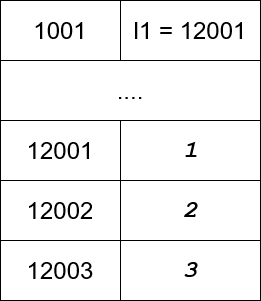
\includegraphics[width=0.2\textwidth]{pointer_diagram_66.png}
    \caption{Memory before call to \texttt{print\_list()}}
    \label{fig:my_label}
\end{figure}\\
Python will copy \texttt{l1} into \texttt{ls} to be the argument of \texttt{print\_list()} using \texttt{=}. Using this information, we can create a memory diagram of the existing variables at the beginning of the function.
\begin{figure}[hbt]
    \centering
    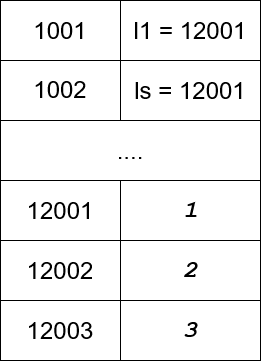
\includegraphics[width=0.2\textwidth]{pointer_diagram_7.png}
    \caption{Memory at start of \texttt{print\_list()}}
    \label{fig:my_label}
\end{figure}\\
Now that the function has been called, \texttt{ls} is no longer just a parameter to write the function \texttt{print\_list()} in terms of, but will now be copy of \texttt{l1} created via \texttt{=}. Thus, \texttt{ls} and \texttt{l1} will both point to 12001. Therefore, changing \texttt{ls[i]} will affect \texttt{l1}, a list that exists outside of the scope of the function \texttt{print\_list()}. \texttt{print\_list()} is not a function that edits the input list as it just prints the list, but I wanted to point out the relationship between an argument that can be referenced by \texttt{ls} and the list that was copied from the calling code \texttt{l1}.
\newpage
\noindent Now, let's write a function that will negate all of the elements \textit{in} the input list. It will not return a new list.
\begin{verbatim}
def negate_list(ls):
    for i in range(len(ls)):
        ls[i] *= -1
\end{verbatim}
This function will set each element in the argument list \texttt{ls} to be the product of its original value with $-1$. Suppose we execute the following code.
\begin{verbatim}
l1 = [1,2,3]
negate_list(l1)
\end{verbatim}
Using Figure 8, \texttt{ls[0] = -1*ls[0] = -1} will really be setting the data at memory location 12001 to $-1$. Similarly, \texttt{ls[1] = -2} and \texttt{ls[2] = -3} will be setting the data at memory location 12002 and 12003 to $-2$ and $-3$ respectively. This is shown in Figure 9.
\begin{figure}[hbt]
    \centering
    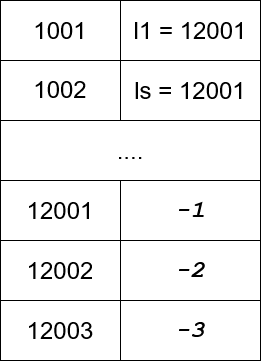
\includegraphics[width=0.2\textwidth]{pointer_diagram_8.png}
    \caption{Memory after \texttt{negate\_list()}}
    \label{fig:my_label}
\end{figure}\\
Now, we can examine the contents of \texttt{l1} using Figure 9. \texttt{l1} still points to the data at location 12001. Thus, we can see that \texttt{l1[0]} is the data at 12001 + 0 which is $-1$. Similarly \texttt{l1[1]} and \texttt{l1[2]} is the data at 12001 + 1 and 12002 which is $-2$ and $-3$ respectively. Thus, we can see that the function \texttt{negate\_list()} actually edits the input argument \texttt{l1} and can see this by printing \texttt{l1}.\\\\
In fact, we can also \texttt{append} to an input list and see the results after the function call in a similar manner. The reason as to why this is true is beyond the scope of this document.

\subsection{Invoking a Function}
For a function that returns no output and does not edit the input, such as \texttt{print\_list()}, we just call it and see the result on the console.
\begin{verbatim}
l1 = [1,2,3]
print_list(l1)
\end{verbatim}
If we have a function that returns something (but does not edit the input), we can store the result of a function in a variable or use it directly. For instance, consider the function \texttt{y(x)}. We can assign the result of \texttt{y} being evaluated at some value to a variable.
\begin{verbatim}
out = y(3)
\end{verbatim}
Or, we can just use the result directly as it is an expression (in particular it's the expression \texttt{3*x + 5} as noted in section 8.1) that will be evaluated by Python. For example, it can be printed directly
\begin{verbatim}
print(y(3))
\end{verbatim}
It can also be used in a boolean condition like any other expression.\\\\
For functions that edit an input, we can call the function on the input and then examine the input (as in the case of \texttt{negate\_input()} above) afterwards.\\\\
Note, we can also have functions that both edit an input and return an output, in which case we would do a combination of the above.

\subsection{Returning Multiple Items}
In Python, you can actually return multiple values from a function. For instance, suppose we want to implement a function \texttt{roots} that returns the positive and negative roots of a number $n$. Using our knowledge of tuples, we could implement it like so
\begin{verbatim}
def roots(n):
    rt = n**0.5
    return (rt, -1*rt)
\end{verbatim}
If we then run
\begin{verbatim}
out = roots(25)
print(type(out))
print(out)
\end{verbatim}
We see the output
\begin{verbatim}
<class 'tuple'>
(5.0, -5.0)
\end{verbatim}
However, we could also write
\begin{verbatim}
def roots2(n):
    rt = n**0.5
    return rt, -1*rt
\end{verbatim}
Then, we can write
\begin{verbatim}
rp, rn = roots2(25)
print(rp, rn)
\end{verbatim}
As we can see here, \texttt{roots2} has 2 separate returned values that can be stored in \texttt{rp} and \texttt{rn}.

\newpage

\section{Reading User Input}
In this section, I will discuss how to read user input from the keyboard in console/command line.

\subsection{The \texttt{input()} Function}
Python provides the function \texttt{input()} which takes a string and returns a string. The string that you pass into it will be displayed to the user as a prompt. The string that is returned is the collection of characters the user entered before they hit the enter/return key. For instance, consider the following code.
\begin{verbatim}
name_in = input("Enter your name! ")
\end{verbatim}
This code will display ``Enter your name! '' on the console and will wait until the user enters some characters and presses the enter key. Then, once the user presses enter, whatever the user input before the enter key will be stored as a string in \texttt{name\_in}.\\\\
It is important to note that since \texttt{input()} returns strings, if we have a program that needs to work with numbers, we will have to make appropriate casts (\texttt{int()} or \texttt{float()}) for instance. 

\subsection{String to List \texttt{(split)}}
A useful function when dealing with user input is the string \texttt{split()} function. For example, suppose we wanted to write a program that asks the user to enter their first name, last name, age, and gender separated by commas. We could prompt and collect this information with the \texttt{input()} function:
\begin{verbatim}
info = input("Enter your first name, last name, age, and gender separated by commas: ")
\end{verbatim}
This will collect the input information into a single string. However, we are more interested in the individual components (first name, last name, age, and gender). Python provides a function \texttt{split()} that will convert a string into a list. \texttt{split()} takes a string as a parameter that tells us which string we want to ``split on''. In this example, we have told the user to separate (or split) the data with commas. Therefore, we can break up \texttt{info} using this code.
\begin{verbatim}
info_list = info.split(",")
\end{verbatim}
For instance, suppose we entered ``John,Smith,20,male'' on the keyboard. This string is stored in \texttt{info}. Then, splitting on ``,'' into \texttt{info\_list} yields \texttt{info\_list} containing
\begin{verbatim}
['John', 'Smith', '20', 'male']
\end{verbatim}
Here we see that we have split up \texttt{info} into the four strings that are separated by the three commas in \texttt{info}.

\newpage

\section{Organizing Code}
In this section, I will discuss some important aspects of organizing code and how it can be implemented in Python.

\subsection{Modularity II (Libraries)}
In section 8.1, I introduced the idea of modularity as the concept of breaking up our program into independent functions. This can be extended further into splitting up our functions into separate files.\\\\
A \textit{library} can be thought of as a collection of general functions. The program that will be run is typically referred to as the \textit{client code}. The client code will use the library functions to perform a more specific application. The client code file is the file you will be running as your program. It will contain a script (code that is not in a function, but will most likely call functions), that will run when you run the file in a Python IDE. It can also contain functions as necessary. 

\subsection{Importing Files}
In Python, all files including library and client code will have the extension \texttt{.py}. Suppose that your client code is in \texttt{main.py} and you have a library of functions \texttt{math\_library.py} that looks like:
\begin{verbatim}
def y(x):
    return 3*x + 5

def z(x,y):
    return 3*x + 2*y + 5
\end{verbatim}
You can import the entire library into \texttt{main.py} by adding the following line to the top of the file.
\begin{verbatim}
import math_library
\end{verbatim}
You can then use the functions from \texttt{math\_library} in \texttt{main.py} in the following manner
\begin{verbatim}
math_library.y(3)
math_library.z(2,3)
\end{verbatim}
We need to precede \texttt{y} and \texttt{z} with \text{math\_library} or Python will think that these functions are defined in \texttt{math.py}. You can import a particular function (such as \texttt{y(x)}) from a file using \texttt{from}-\texttt{import} syntax.
\begin{verbatim}
from math_library import y
\end{verbatim}
You can import multiple functions separated by a comma
\begin{verbatim}
from math_library import y,z
\end{verbatim}
If you have a library file with a particularly long name, Python allows you to provide it with an alias when importing it. 
\begin{verbatim}
import math_library as ml
\end{verbatim}
Then, you can just use \texttt{ml} where you would have used \texttt{math\_library} in \texttt{main.py} in the first example.
\begin{verbatim}
ml.y(3)
ml.z(2,3)
\end{verbatim}

\subsection{Constants II (in Libraries)}
In section 1.4, I mentioned that constants are variables that are not meant to be changed. In Python, there is no way to enforce this, but by naming a variable entirely in uppercase characters conveys to other programmers that these are constants that are not meant to be changed. In math, there is a set of common constants ($e$, $\pi$, etc.). In programs, we use constants quite frequently. Most importantly, constants are used to avoid ``magic numbers''. Magic numbers are any numbers that appear in your program without explanation.\\\\
For instance, suppose you had an environment represented by a two dimensional list. Entries in the 2D list that are 1 represent roads and entries that are 0 represent areas not suitable for travel. For example, we could have an environment that looked like this
\begin{verbatim}
[
    [0, 0, 0, 1, 0, 0, 0], 
    [0, 0, 0, 1, 0, 0, 0], 
    [0, 0, 0, 1, 0, 0, 0], 
    [1, 1, 1, 1, 1, 1, 1], 
    [0, 0, 0, 0, 0, 0, 0], 
    [0, 0, 0, 0, 0, 0, 0], 
    [0, 0, 0, 0, 0, 0, 0]
]
\end{verbatim}
We could initialize this environment using the following code
\begin{verbatim}
environment = []
for i in range(3):
    environment.append([0, 0, 0, 1, 0, 0, 0])
environment.append([1]*7)
for i in range(3):
    environment.append([0]*7)
print(environment)
\end{verbatim}
For this program, I assume that in future we will be moving some entities through the environment and will have to check whether it is travelling on safe ground or not. Or in other words, check if their current position is a 0 or 1. It is better to consider the values in the environment as safe or unsafe. Therefore, it is more appropriate to define constants
\begin{verbatim}
SAFE = 1
UNSAFE = 0
\end{verbatim}
Then, edit our environment creation code
\begin{verbatim}
for i in range(3):
    environment.append([UNSAFE, UNSAFE, UNSAFE, SAFE, UNSAFE, UNSAFE, UNSAFE])
environment.append([SAFE]*7)
for i in range(3):
    environment.append([UNSAFE]*7)
\end{verbatim}
In future code, when we have entities navigating the environment we can check positions to be \texttt{SAFE} or \texttt{UNSAFE}. While this is equivalent to just using 0 and 1, it produces more readable code and allows us to change the representation of safe and unsafe areas in the future.\\\\
The concept of magic numbers applies to other data types. We want to avoid magic strings as well.

\end{document}


